\documentclass{article}
\usepackage[utf8]{inputenc}
\usepackage{mathtools}
\usepackage{amsmath}
\usepackage{amssymb}
\usepackage{witharrows}
\usepackage{cancel}
\newcommand{\norm}[1]{\left\lVert#1\right\rVert}
\newtheorem{definition}{Definition}[section]
\newtheorem{remark}{Remark}[section]
\newtheorem{theorem}{Theorem}[section]


\title{Deep Learning}
\author{Pietro Marcatti}
\date{First Semester 2022/2023}

\begin{document}

\maketitle
\section{History of Deep Learning}
\subsection{Perceptron}
The perceptron algorithm was invented in 1958. The perceptron became the first model for binary classification. It has one weight $w_i$ per input $x_i$. If the result is larger than a threshold it returns 1 otherwise 0 or -1 (non linearity ?).
To train a perceptron we repeat the following steps:
\begin{itemize}
    \item Initialize weigths randomly
    \item Take one sample $x_i$ and predict $y_i$
    \item For erroneous predictions update weights
    \begin{itemize}
        \item If prediction $y = 0$ and ground truth $y_i$ = 1, increase the weights
        \item If prediction $y = 1$ and ground truth $y_i$ = 0, decrease the weights
    \end{itemize}
    \item Repeat until no errors are made
\end{itemize}
However the perceptron can't solve a simple, although non-linear, problem such as the XOR. 
To improve on the perceptron model you must add new layers but there was a stagnation on the neural networks research. The stagnation was caused by a lack of motivation from the community due to the discouraging results of the first perceptron models. 
Still during the AI winter a couple important findings were published such as back-propagation and recurrent neural networks.\\\\
In 2009 the ImageNet dataset was published. It colleted images for each of the 100k terms in WordNet (16M images in total). Terms were organized hierearchally, es: Vehicle \textrightarrow Ambulance.
The ImageNet challange was instituted: 1 million images, 1000 classes, top-5 and top-1 error measured. To build ImageNet they started colleting candidate images from the internet. They then classified the candidates with Amazon Mechanical Turk service.\\
A more recent important achievement was the one obtained by AlphaGo a deep learning model, based on reinforced learning, that in 2016 defeated the best Go player.\\
Deep learning is the first class of learning algorithms that is scalable: performance just keeps getting better as you feed them more data. Instead when working on a small amount of data the performance of a traditional learning model (logistic regression, SVM, decision tree etc) is better.\\
The three key factors for deep learning scaling are:
\begin{itemize}
    \item Data
    \item Computation/hardware
    \item Algorithms
\end{itemize}

\section{Logistic Regression}
Let's start with a simple two feature model:
\begin{itemize}
    \item $x_1$ number of lectures you attend
    \item $x_2$ hours spent on the laboratory activities
\end{itemize}
With logistic regression we want to learn a probabilistic function:
$$\hat{y} = P(y=1|x)$$
In particular the goal is to find the parameters $w$ and $b$ of the following function (hypothesis).
$$H_{w,b}(x)= g =(w^T\cdot x+b) = \frac{1}{1+e^{-(w^T\cdot x+b)}}$$
where $g(z)$ is the sigmoid function so that:
$$\begin{cases}
    H_{w,b}(x) \geq 0.5 & \text{if } y=1\\
    H_{w,b}(x)<0.5 & \text{if } y=0
\end{cases}$$
To get our discrete classification we map the output of the hypthesis function as follow:
$$\begin{cases}
    H_{w,b}(x) \geq 0.5 & \text{\textrightarrow "1"}\\
    H_w,b(x)<0.5 & \text{\textrightarrow "0"}
\end{cases}$$
The decision boundary is $H_{w,b}(x) = 0.5 \rightarrow w^T\cdot x+b=0\rightarrow-3+x_1+2x_2$ supposing we have $b=3$ and $w=[1,2]$. The hypotesis function is $>0.5$ when the argument is $>0$, that is becuause of the shape and output of the sigmoid.

\subsection{Cost Function}
To find $w$ and $b$ so that:
$$\begin{cases}
    H_{w,b}(x) >= 0.5 & \text{if } y=1\\
    H_w,b(x)<0.5 & \text{if } y=0
\end{cases}$$
the logistic classifirer defines the following cost function:
\begin{equation}
    J(w,b) = \frac{1}{m}\cdot \sum_{i=1}^{m}{Cost(h_{w,b}(x^i),y^i)}
\end{equation}
\begin{equation}
    Cost(h_{w,b}(x^i),y^i)= -y^i\cdot ln(h_{w,b}(x^i))-(1-y^i)\cdot ln(1-h_{w,b}(x^i))
\end{equation}
This cost function or loss function is convex and is derivable respect to $w$ and $b$.
In general we call the function to learn the \textbf{hypotesis} but in deep learning it's also called \textbf{model}, while the \textbf{cost function} in deep learning is also called \textbf{loss function}.

\subsection{Gradient Descent}
Gradient descent is a general algorithm for minimizing derivable functions and we are applying it to linear regression.\\
The gradient descent algorithm repeats until convergence the following update on weigths:
\[ 
     \Theta_j = \Theta_j - \alpha \frac{\partial}{\partial\Theta_j}J(\vec{\Theta_0})
\]
It is always necessary to evaluate every new parameter before updating any of them as to not calculate the latters with the new values for the first ones.\\
The hyperparameter $\alpha$ is called the learning rate and it represents the size of the steps that we are taking down the direction of the gradient. For sufficiently small $\alpha$ the cost function should decrease on every iteration. This being said if $\alpha$ is too small it may take a big number of iteration to reach convergence. Finally, a value that is too big for $\alpha$ might cause the cost function to not decrease on every step because we might jump over the "dip", hence it might not converge. It is then a good idea to vary the parameter to experiment with the cost function and its convergence.
\subsubsection{Application of gradient descent on logistic regression}
Once we've established our decision function, in this example the logistic regression, we can procede to apply the gradient descent. To do that we first need to calculate the partial derivatives of the Loss function with respect to every parameter ($\vec{w}$ and $\vec{b}$) so that we can apply the changes. In this example with two inputs:
\begin{align*}
    w_1 &:= w_1 - \alpha \frac{\partial J(\vec{w},\vec{b})}{\partial w_1}\\
    w_2 &:= w_2 - \alpha \frac{\partial J(\vec{w},\vec{b})}{\partial w_2}\\
    b &:= b - \alpha \frac{\partial J(\vec{w},\vec{b})}{\partial b}\\
\end{align*}

\section{Neural Networks}
Neural Networks expand on the simple ideas of perceptron computing units by adding more layers on neurons betweeen the input and the output. As the shape of the neural network changes so does the way we represent it:
\begin{itemize}
    \item $W^{[j]}$: its the matrix of weights controlling the function mapping from layer j-1 to layer j
    \item $b^{[j]}$: the value of the bias for the j-th layer
    \item $a^{[j]}$: activation vector for the layer j
    \item $g^{[j]}$: activation function for the layer j
\end{itemize}
\subsection{Activation Functions}
In deep neural networks you also have to specify what activation function you want to apply to the activation vectors of each hidden layer. In the hidden layers we rarely see the sigmoid function because it is said to kill the gradient. This refers to the fact that the sigmoid, for particularly large or small inputs, saturates at 1 or 0 respectively. The hyperbolic tangent also suffers from this vanishing gradient problem but it generally performs better than the sigmoid. The sigmoid function is still widely used in the output or final layer to give a probabilistic meaning to our output as it's betweeen [0,1].\\
What are other types of activation function that we can be used in the hidden layers?
\begin{description}
    \item[ReLU or Rectified Linear Unit]:
        It's particularly easy to train and achieves great performance. Its derivative is particularly easy to calculate, given that you consider the point of non-derivability in 0. 
    \item[Leaky ReLU]: Leaky ReLU was created to solve the dying ReLU problem which affects neuron with ReLU activation functions. If their parameter is stuck at 0 no matter the input their output will be 0. If this happens no gradient flows and there cannot be any learning. To avoid this it assigns a slightly sloped straight line for the negative values.
\end{description}
It is fundamental to use non-linear activation functions otherwise the output of the neural network will be a simple linear combination of the inputs. Let's suppose our activation function is the identity function: $ g^{[1]}(z) = g^{[2]}(z) = z $ 
\[ 
    a^{[2]} = z^{[2]}= W^{[2]}a^{[2]}+b^{[2]} =  W^{[2]}(W^{[1]}x+b^{[1]})+b^{[2]} = (W^{[2]}W^{[1]})x + (W^{[2]}b^{[1]}+b^{[2]})
\]
We can define $ W' = W^{[2]}W^{[1]} $ and $ b'= W^{[2]}b^{[1]}+b^{[2]}$ then we can rewrite $ a^{[2]} = W'x +b'$. Linear activation function is then useless unless in the last layer when performing a regression task.
\subsection{Back propagation}
Back propagation is the concept and algorithm that allows to update the weights of the neural network to learn. It relies on two simple steps:
\begin{description}
    \item[Forward Step:] in this step is activated on one example and the error of each neuron of the output layer is computed.
    \item[Backwards Step:] in this step the network error is used for updating the weights. Starting at the output layer, the error is propagated backwards through the network layer by layer. This is done recursively computing the local gradient of each neuron.  
\end{description}
\begin{definition}[Jacobian Matrix]
    The derivative of a vector function (a vector whose components are functions) with respect to an input vector x is called a Jacobian Matrix and is represented as:
    \[ 
        \frac{\partial y}{\partial x}=
        \begin{bmatrix}
            \frac{\partial y_1}{\partial x_1} & \cdots & \frac{\partial y_1}{\partial x_n} \\
            \vdots & \ddots & \vdots \\
            \frac{\partial y_m}{\partial x_1} & \cdots & \frac{\partial y_m}{\partial x_n} \\
        \end{bmatrix}
    \]
    
\end{definition}
It is particularly important to set a reasonable initial value for the weights. If we used 0 on all weights, all $ z^{[1]} $ would be 0, hence $ a^{[1]}_1 = \ldots =a^{[1]}_n $ because we would always get the same mapping by the activation function. The derivaties used to obtain the gradient would be equal and so the weights and bias would all be changed by the same amount remaining all equal. We refer to this phenomenon as the symmetry problem and to counter it we can simply initialize the weights to a small random value. The reason for such a small value has to do with the previously mentioned vanishing problem. If your network starts working with big numbers it will get to the sigmoid in the output layer and be saturated on the 1 or 0 with very little gradient to move.

\subsection{Hyperparameters}
We've already referred to some of our variables as hyperparameters. We can identify an hyperparameter by considering if it is a variable that can be changed to impact the functioning and the performance of our model without it being a parameter such as the weights and the bias. Examples of hyperparameters are:
\begin{itemize}
    \item Learning rate
    \item Number of interaction (or epochs)
    \item Number of hidden layers
    \item Number of hidden units in each hidden layers
    \item Activation functions
\end{itemize}
The process of tuning these values to achieve the best result is for us, right now, all empirical.

\section{Improving our Neural Network}
In the process of training our neural network we often divide all the data we have available in two or three sets. These are the training and test set, plus optionally, the validation set. The training set contains the data we use to perform the learning of our model. If available we then measure the performance on the validation set in real world mock-up scenario. Eventually, when our model is stable we test it on the test set to get a real measure of it's performance.\\
It is fundamental that validation and test have the same distribution to ensure meaningful learning.\\
We divide our training data set into smaller batches of usually around 16-32-64 samples. We compute forward and backwards on every single sample. Once we complete all the batches we completed an epoch. We can then start again but now, on the first batch, our neural network will have weights that will have already changed thanks to all other batches.

\subsection{Overfit vs. Underfit}

\subsubsection{Regularization}
Logistic Regression: Minimization problem with regularization:$ \;\min_{w,b}{J(w,b)}$
$$J(w,b)= \frac{1}{m}\left[ \sum_{i=1}^{m}{Cost(h_{w,b}(x^{(i)}), y^{(i)})+\frac{\lambda}{2}\sum_{j=1}^{n}{w_i^2}} \right]$$
$\lambda$ is called the regularization parameter, usually b is ignored in the regularization process.
By setting a big regularization parameter we are saying that our minimization algorithm should focus on reducing the weights. The goal is to have the weights all in the same order of magnitude.\\\\
Doesn't regularization kill the importance of some features over others?\\\\
Regularization with Neural Networks:\\
$$J(W^{[1]}, b^{[1]}W^{[2]}, b^{[2]})= \frac{1}{m}\left[ \sum_{i=1}^{m}{\mathbb{L}(\hat{y}, y^{(i)})+\frac{\lambda}{2}\sum_{i=1}^{L}{\norm{W^{[l]}}^2_F}} \right]$$

Where $\lambda$ is the regularization parameter, l is the layer. $$\norm{W^{[i]}}^2_F=\sum_{i=1}^{n{[l-1]}}{\sum_{j=1}^{n^{[l]}}{(W_{i,j}^{[l]})^2}}$$
Where $W^{[l]}\in \mathbb{R}^{n^{[l]}\times n^{[l-1]}}$\\
Regularization helps preventing overfitting because by using a big value for $\lambda$ we minimize weigths close to 0 and some of them are basically dead (almost 0)\\\\
Too many dead nodes means underfitting? Would it ever be useful to have a small $\lambda$\\\\

\subsection*{Vanishing and Esploding Gradients}
We can observe this phenomenon when dealing with very deep neural networks. In summary, we want to initialize the weights around 1, otherwise through repeated multiplication we would end up with very large or extremely small numbers in the weights matrix. 


\subsection{Normalization}
Mean normalization transforms dta to have a mean of zero and a standard deviation of 1. Such normalization is the preferred normalization for Neural Networks. Given a feature $ x_i $ the mapped feature is $ x^i  = \frac{x_i-\mu_i}{\sigma_i}$ where $ \mu_i, \sigma_i $ are the mean and standard deviation computed on the training set. It is important to normalize each feature separately as its data come from different distributions and the feature number is exactly what the index $ x_i $ refers to.\\
The MinMaxNormalization shifts the data such that all features are exactly between 0 and 1. 
\[ 
    x_{i}^{'}= \frac{x_i-\min{x}}{\max{x} - \min{x}} 
\]
It's very important to apply the same transformation to the trainin set and the test set for the supervised model to work on the test set. The figure illustrates what would happen if we were to use the minimum and range of the test set instead.
\begin{figure}[htbp]
    \centering
    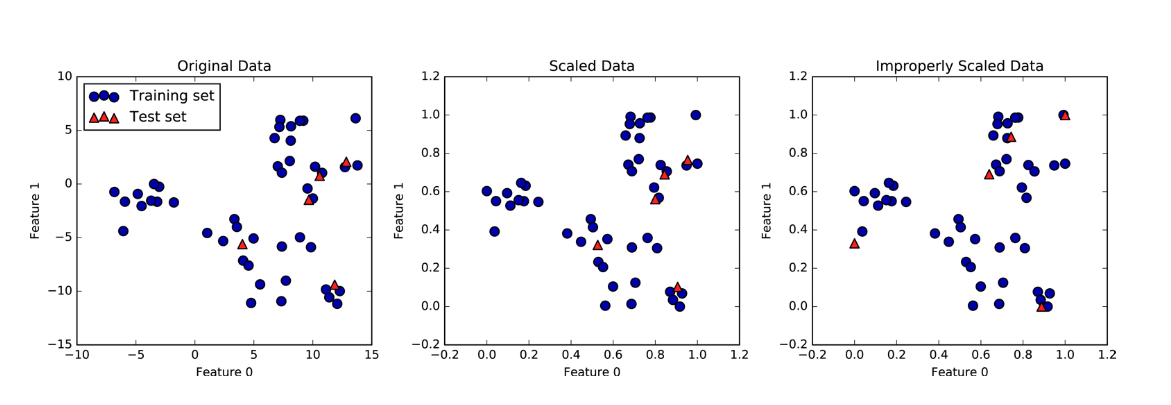
\includegraphics[width=13cm]{normalization-effect.png}
\end{figure}
The correct procedure is to normalize the training set and then once we have a stable model we can normalize also the test set with the same min and max values computed for the training set.

\section{NLP and Word Embedding}
Natural language processing is a field of deep learning in which you focus on recognizing elements of written text speech particles. Other fields of use are the summarization of text, question answering, automatic email response and forwarding, chatbots ecc ecc\\
Word embedding is a field of deep learning. It aims to represent a word as feature vectors, and consequently as numbers. The simplest way is to assign each word of a vocabulary a number but this way you could sort words which doesn't map as a semantic characterstic for words. A different way is to use a one-hot vector for each words. These vectors are the size of the vocabulary and only for the word we want to represent we put 0 in the corresponding position, otherwise 0. This representation has some pros: it's simple and it doesnt imply ordering. The cons: huge vectors and no embedded meaning.\\
The next idea is to represent words in a semantic space through vectors that can carry the essence of the meaning. We could, for example, place words on a real scale where the negative half expresses how negative the essence of the word is on the contrary the positive axis imply positivity.\\ We could expand this model to include two dimensions, they could for example represent how abstract or, inversely, concrete a word is. This kind of representation is defintely a step up and we have a low dimensionality representation for words and there is an embedded meaning from which to derive semantic distance or closeness.
\subsection*{Word embedding process}
We take a corpus (be it general purpose or specialized for a given context). The embedding algorithm will use a high feature space (around 300) to try and position the words of the corpus in such space. We then want to validate the goodness of the model by using it in NLP tasks.\\
\subsubsection*{Word2Vec algorithm}
Is a technique for builiding a rich semantic word embedding space (by google 2013). The key idea is to have similar embeddings for words that have similar meaning and context.It works by creating a fake task: given a specific word in the middle of a sentence (the input word), the network is going to tell us the probability for every word in our vocabulaty of being near-by the word we chose. The "near-by" amount is a parameter that we define, usually 5 before and 5 after the input word. \\
The resulting neural network is composed by input, one hidden and output layer. There is no activation function on the hidden layer neurons. The dimensionality of the hidden layer is equal do the dimensionality of the embeddin (example 300)


\section{Exercises}
\renewcommand{\arraystretch}{1.5}
\subsection*{Neural Network}
\subsubsection*{Exercise 1}
Consider the following neural network which takes two binary-valued inputs $x_1,x_2 \in {0,1}$ and outputs $h_\theta(x)$. Which of the following logical function does it compute?
\begin{figure}[htbp]
    \centering
    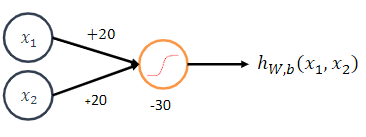
\includegraphics[width=10cm]{ExerciseBook/01-NeuralNetwork/exercise1.png}\newline
\end{figure}\newline
To anser we can simply compute the truth table for the possible values of $x_1, x_2$.
\begin{center}
    
    \begin{tabular}{ |c |c |c |}
        \hline
        \textbf{$x_1$} & \textbf{$x_2$} & \textbf{$h_{W,b}(x_1,x_2)$} \\
        \hline
        0 & 0 & -30 (0) \\ 
        0 & 1 & -10 (0) \\  
        1 & 0 & -10 (0) \\
        1 & 1 & 10 (1)\\
        \hline
    \end{tabular}
    Answer: logical AND
\end{center}
\subsubsection*{Exercise 2}
Consider the following neural network:
\begin{figure}[htbp]
    \centering
    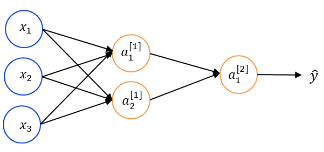
\includegraphics[width=10cm]{ExerciseBook/01-NeuralNetwork/exercise2.png}\newline
\end{figure}
I start by computing the activation vector $z^{[1]}$ by multiplying $W\cdot x+b^{[1]}$.
\[ 
    z^{[1]}=
    \begin{bmatrix}
        -1 \\
        8 
    \end{bmatrix}
\]
\\I then plug the activation vector into the activation function to get $a^{[1]} = g(z^{[1]}) = \frac{1}{1-e^{-z^{[1]}}}$
\[ 
    a^{[1]}=
    \begin{bmatrix}
        0.268941 \\
        0.999665
    \end{bmatrix}
\]\\I repeat for the next layer
\[ 
    z^{[2]}=
    \begin{bmatrix}
        2.537547
    \end{bmatrix}
\]
\\We conclude $a^{[2]}=0.926732$
\subsubsection*{Exercise 3}
\begin{figure}[htbp]
    \centering
    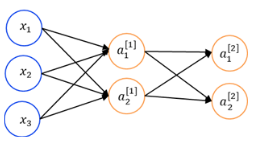
\includegraphics[width=10cm]{ExerciseBook/01-NeuralNetwork/exercise3.png}\newline
\end{figure}
I start by computing the activation vector $z^{[1]}$ by multiplying $W\cdot x+b^{[1]}$.
\[ 
    z^{[1]}=
    \begin{bmatrix}
        4 \\
        -16
    \end{bmatrix}
\]
\[ 
    a^{[1]}=
    \begin{bmatrix}
        0.982014 \\
        0.00000012 \\ 
    \end{bmatrix}
\]
\[ 
    z^{[2]}=
    \begin{bmatrix}
        2.964028 \\
        3.964027
    \end{bmatrix}
\]
\[ 
    a^{[2]}=
    \begin{bmatrix}
        0.268941 \\
        0.731058
    \end{bmatrix}
\]
\subsubsection*{Esercise 4}
In this diagram which we hand-drew in lecture, what do the horizontal axis (x-axis) and vertical axis (y-axis) represent?
\begin{figure}[htbp]
    \centering
    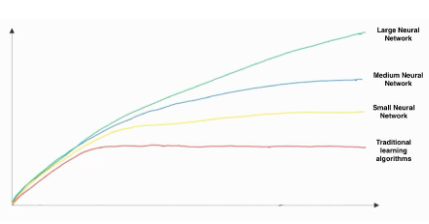
\includegraphics[width=10cm]{ExerciseBook/01-NeuralNetwork/exercise4.png}\newline
\end{figure}
Answer: x-axis is the amount of data; y-axis (vertical axis) is the performance of the algorithm.
\subsubsection*{Exercise 5}
Which one of these plots represents a ReLU activation function?
\begin{figure}[htbp]
    \centering
    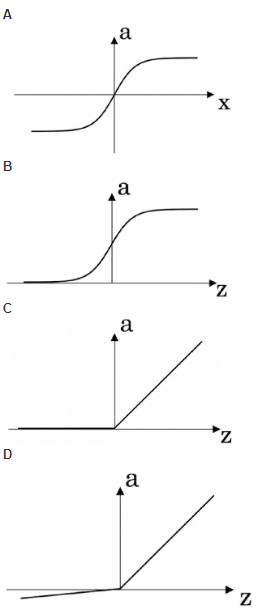
\includegraphics[width=6cm]{ExerciseBook/01-NeuralNetwork/exercise5.png}\newline
\end{figure}
Solution answer C
\subsubsection*{Exercise 6}
Which of these is the "Logistic Loss"?\\
Solution answer A
\subsubsection*{Exercise 7}
Consider the following computation graph. What is the output J?
\begin{figure}[htbp]
    \centering
    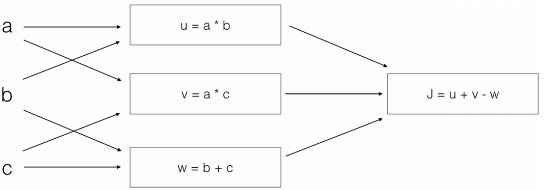
\includegraphics[width=12cm]{ExerciseBook/01-NeuralNetwork/exercise7.png}\newline
\end{figure}
Solution answer B
\subsubsection*{Exercise 8}
You are building a binary visual classifier for recognizing apples(y=1) vs. tomatoes(y=0). Which one of these activation functions would yourecommend using for the output layer?
\\Solution: answer C : Sigmoid because it's perfect for linear classification between [0,1]
\subsubsection*{Exercise 9}
Suppose you have built a neural network. You decide to initialize the weights and biases to be zero. Which of the following statements is true?\\
Solution answer A: Each neuron in the first hidden layer will perform the same computation. So even after multiple iterations of gradient descent each neuron in the layer will becomputing the samething as other neurons.
\subsubsection*{Exercise 10}
Consider the following 2 hidden layer neural network, which of the following statements are True?
\begin{figure}[htbp]
    \centering
    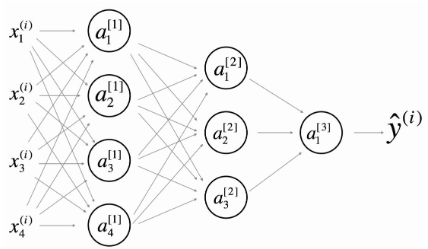
\includegraphics[width=12cm]{ExerciseBook/01-NeuralNetwork/exercise10.png}\newline
\end{figure}
Solution, answers A, B, F
\subsubsection*{Exercise 11}
The dev and test set should:
Solution answer A: come from the same distribution.
\subsubsection*{Exercise 12}
If your Neural Network model seems to underfit your data, what of the following would be promising things to try?\\
Solution answers: B, C
\end{document}
